\documentclass[journal,10pt,twocolumn]{IEEEtran}

\usepackage[utf8]{inputenc}
\usepackage{amsmath,amssymb,amsfonts}
\usepackage{graphicx}
\usepackage{booktabs}
\usepackage{array}
\usepackage{cite}
\usepackage{url}
\usepackage{hyperref}
\usepackage{listings}
\usepackage{color}

\hypersetup{
    colorlinks=true,
    linkcolor=blue,
    citecolor=blue,
    urlcolor=blue
}

\begin{document}

\title{Phase I Technical Report: Design and Implementation of a 2-Way Set-Associative Cache with True LRU Replacement Compared Against a Direct-Mapped Baseline}

\author{
    Member~1 (Team Lead \& 2-Way RTL),
    Member~2 (LRU Logic \& Verification),
    Member~3 (Direct Baseline \& Memory),
    Member~4 (Traces \& Benchmarks),
    and~Member~5 (Report, Diagrams, Synthesis \& Video Lead)\\
    \textit{Project 7: Cache Memory Subsystem Design (Phase I) | MCA Capstone}
}

\maketitle

\begin{abstract}
This report presents the architectural design, cycle-accurate simulation, and comparative evaluation of a 1024-Byte (1~KB) 2-way set-associative level-1 data cache against an identically sized direct-mapped baseline. Both microarchitectures are implemented in synthesizable Verilog HDL with a 16-Byte block size (4 words of 32 bits each), interfacing with a 32-bit CPU bus and a parameterized backing main memory controller under a Write-Through No-Write-Allocate coherence policy. The 2-way cache employs a true Least Recently Used (True LRU) replacement algorithm implemented via a dedicated single-bit-per-set status array, invalid-way priority allocation, and parallel continuous tag comparison. Across a suite of nine deterministic synthetic memory access workloads totaling 3,136 transactions, zero data mismatches were observed against an architectural golden memory model. Experimental evaluation demonstrates the canonical advantage of set associativity on conflict-heavy workloads: under the ping-pong access pattern, the 2-way cache achieves a 99.00\% hit rate (424 clock cycles) compared to 0.00\% (2,800 clock cycles) for the direct-mapped cache, representing a 6.6$\times$ execution speedup. Conversely, on pathological access patterns exceeding set capacity, both designs experience severe degradation: under 3-way cyclic traversal (\texttt{cyclic3}), both suffer 0.00\% hit rates (4,200 cycles). On a 1.5~KB loop exceeding capacity (\texttt{large\_loop}), the direct-mapped cache paradoxically outperforms the 2-way cache (25.00\% vs 0.00\% hit rate, 4,224 vs 5,376 cycles) due to partial line survival across modulo-64 line mappings. Synthesis trade-offs, storage array register allocation, and unbuffered write stalls are analyzed.
\end{abstract}

\begin{IEEEkeywords}
Cache memory, set-associative cache, direct-mapped cache, True LRU, write-through, memory hierarchy, Verilog HDL, cycle-accurate simulation.
\end{IEEEkeywords}

\section{Introduction}
The expanding performance disparity between high-performance microprocessor execution pipelines and relatively high-latency dynamic RAM (the memory wall) mandates efficient on-chip cache memory subsystems. Caches mitigate memory latency by exploiting two fundamental locality principles: spatial locality (the likelihood that references near recently accessed data will soon be needed) and temporal locality (the likelihood that recently accessed data will be re-referenced in the near future)~\cite{hennessy2017,smith1982cache}.

In microprocessor architecture, set associativity represents a core design choice balancing miss rate reduction against hardware complexity and critical path timing~\cite{hennessy2017,hill1989evaluating}. Direct-mapped caches require minimal control logic and only a single tag comparator, offering rapid lookup latency and minimal energy overhead per access. However, because each memory address maps to exactly one predetermined cache line based on its index bits, direct-mapped caches suffer severely from conflict misses when multiple frequently referenced working-set blocks share the same cache line~\cite{jouppi1990improving}. Set-associative caches alleviate conflict thrashing by allowing a memory block to reside in any of $N$ ways within a designated set, but introduce parallel tag comparators, hit-way multiplexing, and replacement policy tracking logic~\cite{hennessy2017,hill1989evaluating}.

The objective of Phase I of Project 7 is to design, implement, and rigorously benchmark a 1~KB 2-way set-associative data cache with True LRU replacement against an identically sized 1~KB direct-mapped baseline in Verilog HDL. To ensure strict fairness, both architectures maintain identical user storage capacity (1024 Bytes), identical block size (16 Bytes / 4 words), identical 32-bit microprocessor byte-address interfaces, and identical backing memory timing parameters. Through extensive cycle-accurate simulation across nine synthetic traces exercising spatial locality, temporal loops, set conflicts, cyclic thrashing, pseudorandom access, and mixed read/write traffic, we evaluate the precise architectural trade-offs between conflict immunity, replacement policy limitations, and hardware resource utilization.

\section{Literature Review}
The theory and empirical evaluation of cache memory subsystems have been extensively investigated in computer architecture literature:

\begin{enumerate}
    \item \textbf{Miss Classification and Associativity Principles:} Hennessy and Patterson~\cite{hennessy2017} formulated the classical ``3Cs'' taxonomy of cache misses: compulsory misses (cold starts occurring upon the first reference to a memory block), capacity misses (arising because the cache cannot contain all blocks needed during program execution), and conflict misses (occurring when multiple blocks compete for the same set in direct-mapped or set-associative designs). Set associativity specifically eliminates conflict misses by providing alternative storage slots within each set, approaching the miss rate of a fully associative cache of identical capacity~\cite{hennessy2017}.
    \item \textbf{Foundational Replacement and Design Trade-offs:} In his seminal survey, A. J. Smith~\cite{smith1982cache} comprehensively analyzed cache memory structures, line sizing, and replacement algorithms. Smith established that Least Recently Used (LRU) replacement consistently yields superior or near-optimal hit ratios among online non-lookahead replacement strategies by directly capturing temporal locality in referenced working sets.
    \item \textbf{Stack Algorithms and LRU Optimality:} Mattson et al.~\cite{mattson1970evaluation} proved that LRU belongs to the class of inclusion-property ``stack algorithms.'' In a stack algorithm, the contents of an $N$-way cache are guaranteed to be a strict subset of the contents of an $(N+1)$-way cache for any given reference string, precluding anomalous hit-rate degradation when increasing cache size. However, Mattson et al. also documented the known vulnerability of finite-stack LRU policies to cyclic access sequences where the working set strictly exceeds associativity by one block ($N+1$).
    \item \textbf{Quantifying Associativity Benefits:} Hill and Smith~\cite{hill1989evaluating} introduced trace-driven simulation techniques to isolate the performance impact of associativity. Their empirical findings showed that shifting from a direct-mapped cache to a 2-way set-associative cache provides the single largest marginal reduction in conflict misses, whereas increasing associativity further (to 4-way or 8-way) provides diminishing returns while introducing significant clock-cycle hit-time penalties.
    \item \textbf{Conflict Miss Vulnerability of Direct-Mapped Caches:} Jouppi~\cite{jouppi1990improving} demonstrated that the majority of miss penalties in direct-mapped caches stem from a small number of conflicting lines that repeatedly ping-pong. Jouppi proposed auxiliary structures such as victim caches to address conflict misses without incurring the multiplexing latency of fully set-associative designs, reinforcing the critical need to quantify conflict behavior.
\end{enumerate}

\section{Proposed Solution}

\subsection{Cache Parameters and Address Decomposition}
To ensure a strictly fair comparison between the 2-way set-associative cache and the direct-mapped baseline, both architectures are sized for an identical user data capacity of \textbf{1024 Bytes (1~KB)} and an identical block size of \textbf{16 Bytes (4 words of 32 bits each)}. Both designs interface with a standard 32-bit microprocessor byte address.

\begin{table}[htbp]
\centering
\caption{Architectural Parameter Derivations and Comparison}
\label{tab:params}
\begin{tabular}{p{2.6cm}p{2.3cm}p{2.3cm}}
\toprule
\textbf{Parameter} & \textbf{2-Way Set-Assoc.} & \textbf{Direct-Mapped} \\
\midrule
User Data Capacity & 1024 Bytes (1 KB) & 1024 Bytes (1 KB) \\
Block Size (Burst Unit) & 16 Bytes (4 words) & 16 Bytes (4 words) \\
Associativity (Ways/Set) & 2 Ways & 1 Way (Direct-Mapped) \\
Total Sets / Lines & 32 Sets & 64 Lines \\
Block Offset Width & 4 bits (\texttt{addr[3:0]}) & 4 bits (\texttt{addr[3:0]}) \\
Word Select Bits & 2 bits (\texttt{addr[3:2]}) & 2 bits (\texttt{addr[3:2]}) \\
Byte Offset Bits & 2 bits (\texttt{addr[1:0]}) & 2 bits (\texttt{addr[1:0]}) \\
Set Index Width & 5 bits (\texttt{addr[8:4]}) & 6 bits (\texttt{addr[9:4]}) \\
Tag Width & 23 bits (\texttt{addr[31:9]}) & 22 bits (\texttt{addr[31:10]}) \\
Valid Storage Bits & 64 bits ($32 \times 2$) & 64 bits ($64 \times 1$) \\
LRU Replacement Bits & 32 bits ($32 \times 1$) & 0 bits \\
\bottomrule
\end{tabular}
\end{table}

\textbf{Why the Tag Width Differs:} In the 2-way cache, grouping two lines into each set halves the total number of sets from 64 to 32. Halving the set count reduces the index field from 6 bits to 5 bits. Because the total address is fixed at 32 bits and the block offset remains 4 bits, the unused index bit shifts into the tag field, increasing tag width from 22 bits to 23 bits.

\subsection{Hardware Architecture \& Datapath}
The 2-way set-associative cache datapath consists of two parallel storage ways (Way~0 and Way~1), parallel continuous tag comparators, hit-way multiplexing logic, a True LRU tracking array, and memory bus interfacing logic.

\begin{figure}[htbp]
\centering
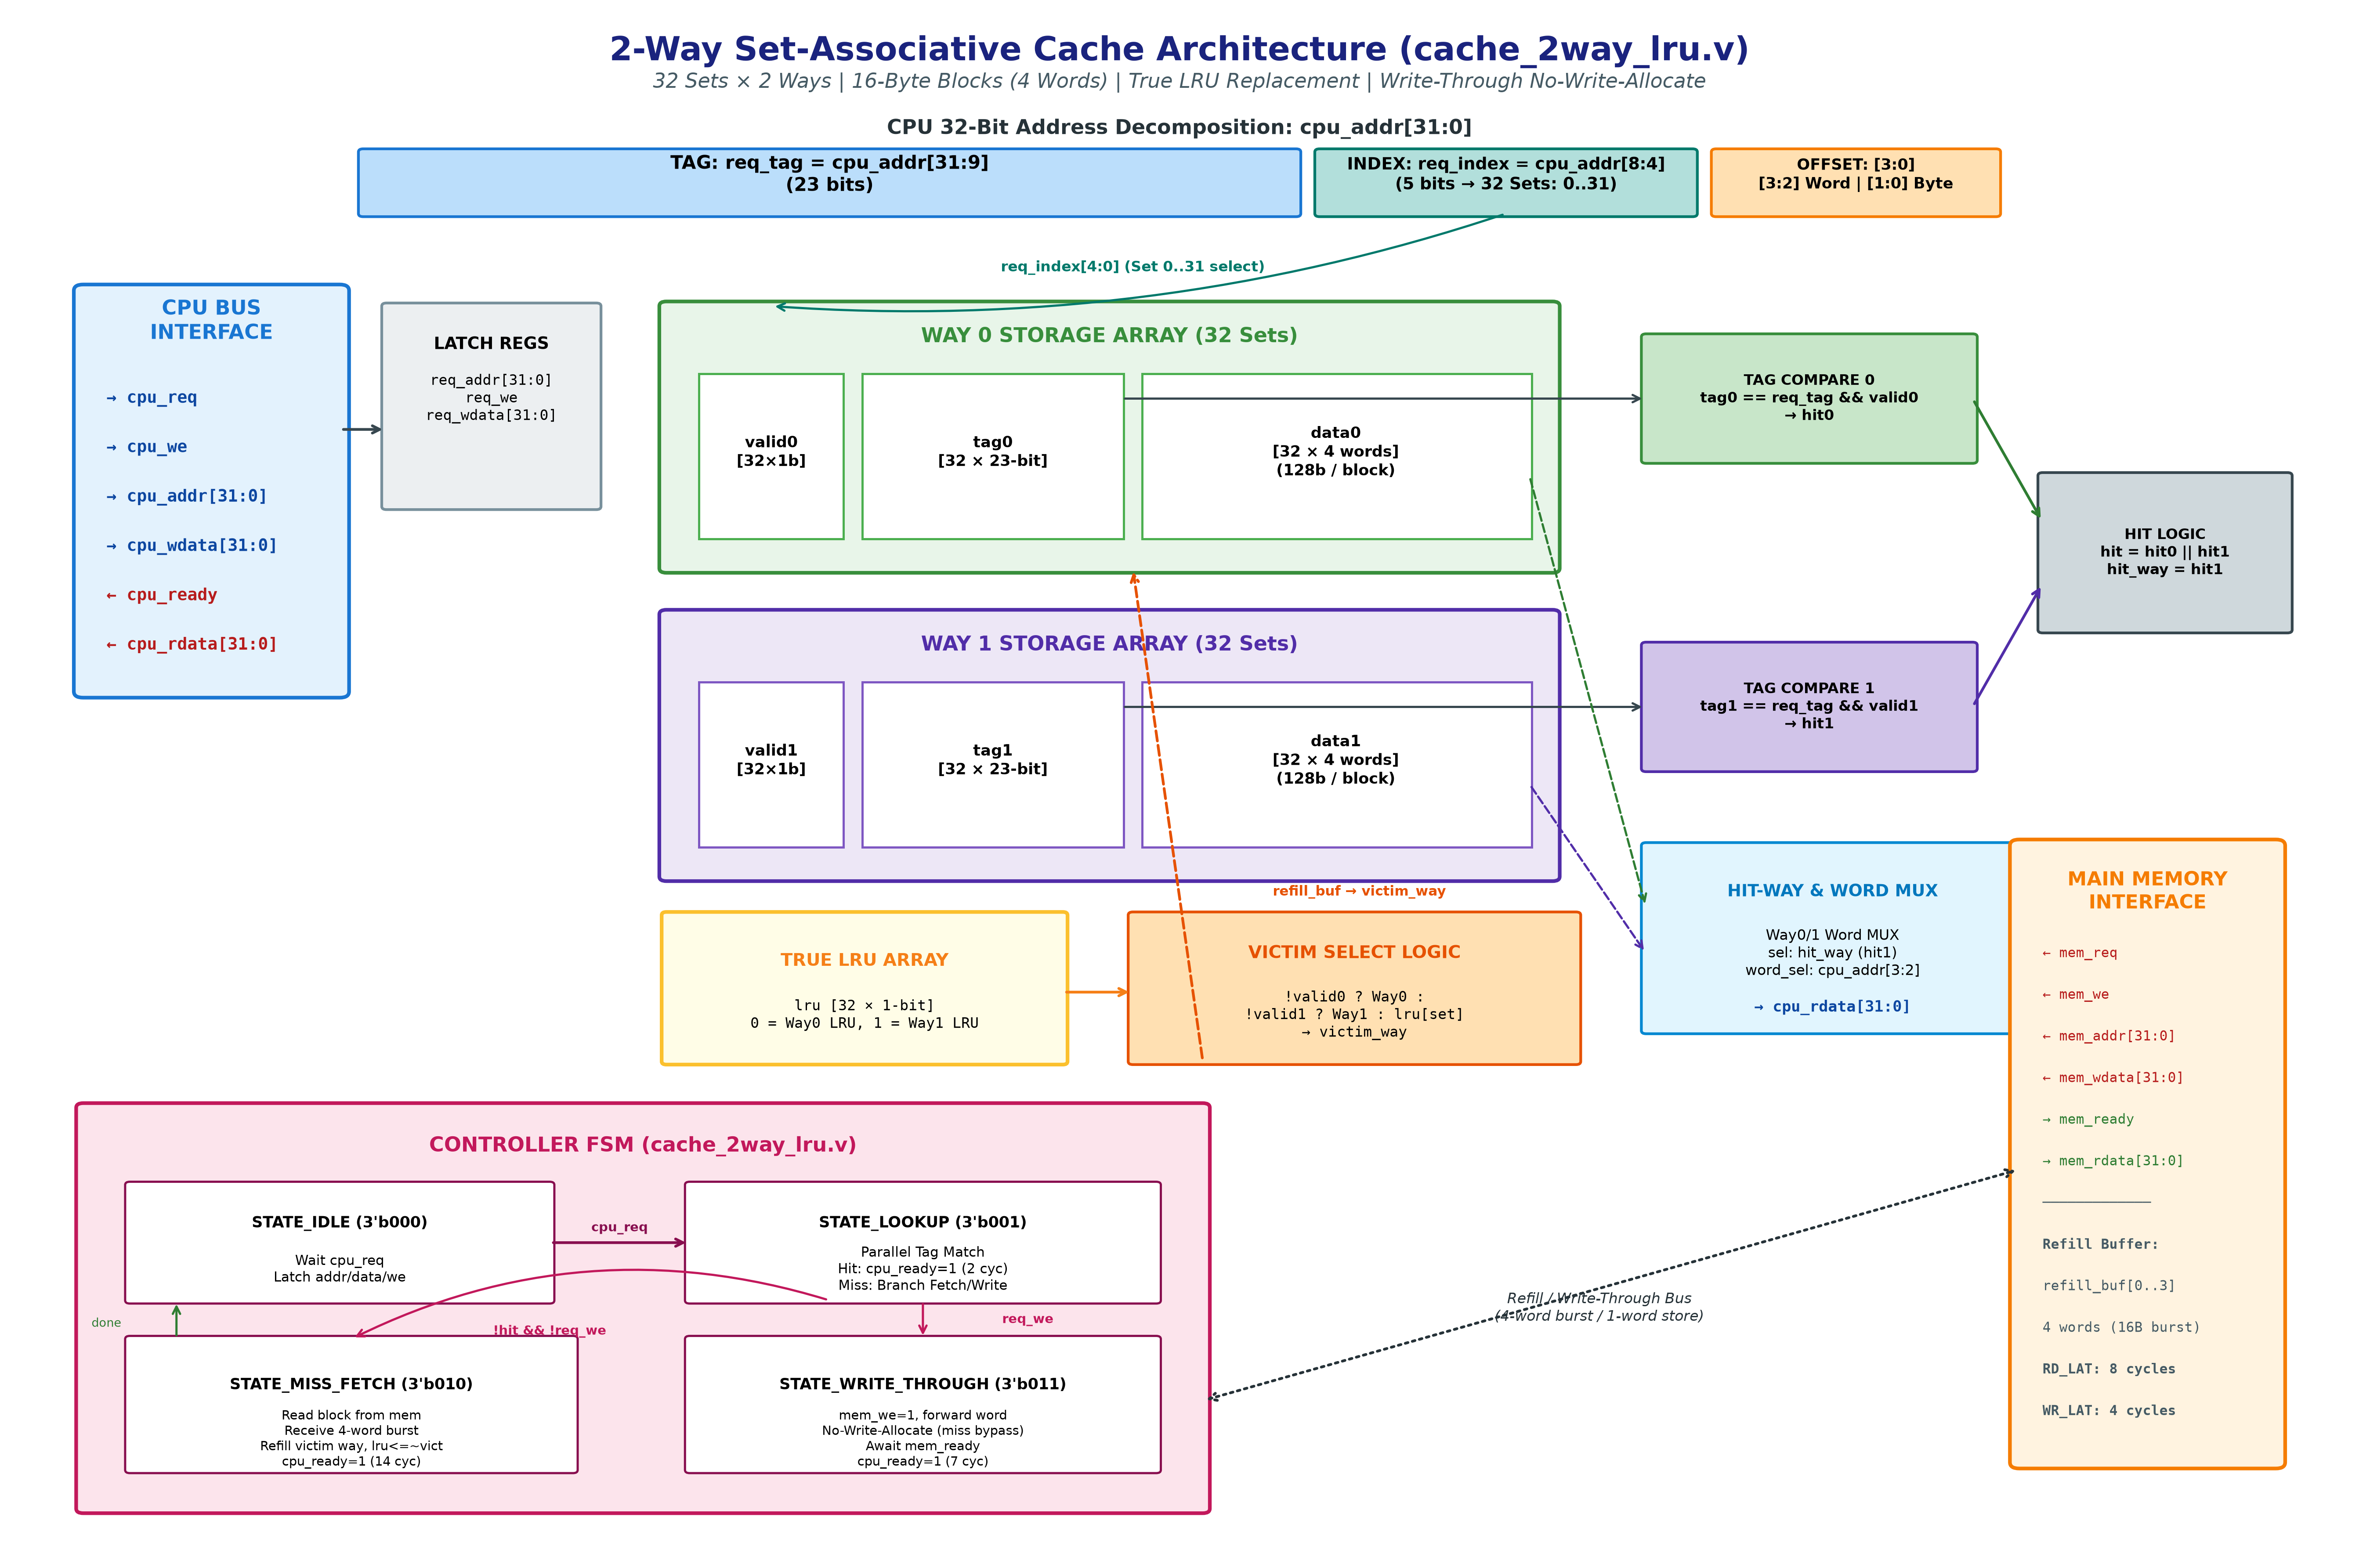
\includegraphics[width=\columnwidth]{block_diagram.png}
\caption{Complete microarchitectural block diagram of the 2-way set-associative cache controller and datapath (\texttt{cache\_2way\_lru.v}). Generated via script \texttt{scripts/make\_block\_diagram.py}; may be redrawn in draw.io for submission.}
\label{fig:block_diagram}
\end{figure}

The datapath elements operate as follows:
\begin{itemize}
    \item \textbf{Storage Arrays:} Each of the 32 sets maintains storage for both ways: \texttt{valid0} and \texttt{valid1} (32$\times$1b), \texttt{tag0} and \texttt{tag1} (32$\times$23b), and \texttt{data0} and \texttt{data1} (32$\times$4$\times$32b = 128b/block).
    \item \textbf{Parallel Comparators:} Continuous assignments evaluate both tags simultaneously:
    \begin{align*}
        \texttt{hit0} &= \texttt{valid0[req\_index]} \land (\texttt{tag0[req\_index]} == \texttt{req\_tag}) \\
        \texttt{hit1} &= \texttt{valid1[req\_index]} \land (\texttt{tag1[req\_index]} == \texttt{req\_tag}) \\
        \texttt{hit}  &= \texttt{hit0} \lor \texttt{hit1}, \quad \texttt{hit\_way} = \texttt{hit1}
    \end{align*}
    \item \textbf{Hit-Way Multiplexer:} Selects the requested 32-bit data word from Way~0 or Way~1 based on \texttt{hit\_way}.
\end{itemize}

\subsection{True LRU Replacement Logic}
With two ways per set, a miss in a full set forces the cache to choose which resident block to evict. The architecture implements true Least-Recently-Used (LRU) replacement: the evicted block is always the block accessed longest ago in logical time.

\begin{itemize}
    \item \textbf{State Representation:} Each set keeps exactly one LRU bit, \texttt{lru[set]}, encoding the victim way: \texttt{0} indicates Way~0 is LRU; \texttt{1} indicates Way~1 is LRU. One bit per set fully captures the recency order of 2 ways ($2! = 2$).
    \item \textbf{Update Rules:} On a read hit or write hit in way $w$, \texttt{lru <= \textasciitilde w}. On a block refill into victim way $v$, \texttt{lru <= \textasciitilde v}. On a write miss under No-Write-Allocate, cache state is untouched.
    \item \textbf{Victim Selection Priority:} The controller prioritizes invalid ways before consulting the LRU bit:
    \begin{align*}
        \texttt{victim\_way} = (\neg\texttt{valid0}) \,?\, 0 : ((\neg\texttt{valid1}) \,?\, 1 : \texttt{lru})
    \end{align*}
    Invalid lines are populated first, ensuring valid data is never evicted while empty ways exist.
\end{itemize}

\begin{figure}[htbp]
\centering
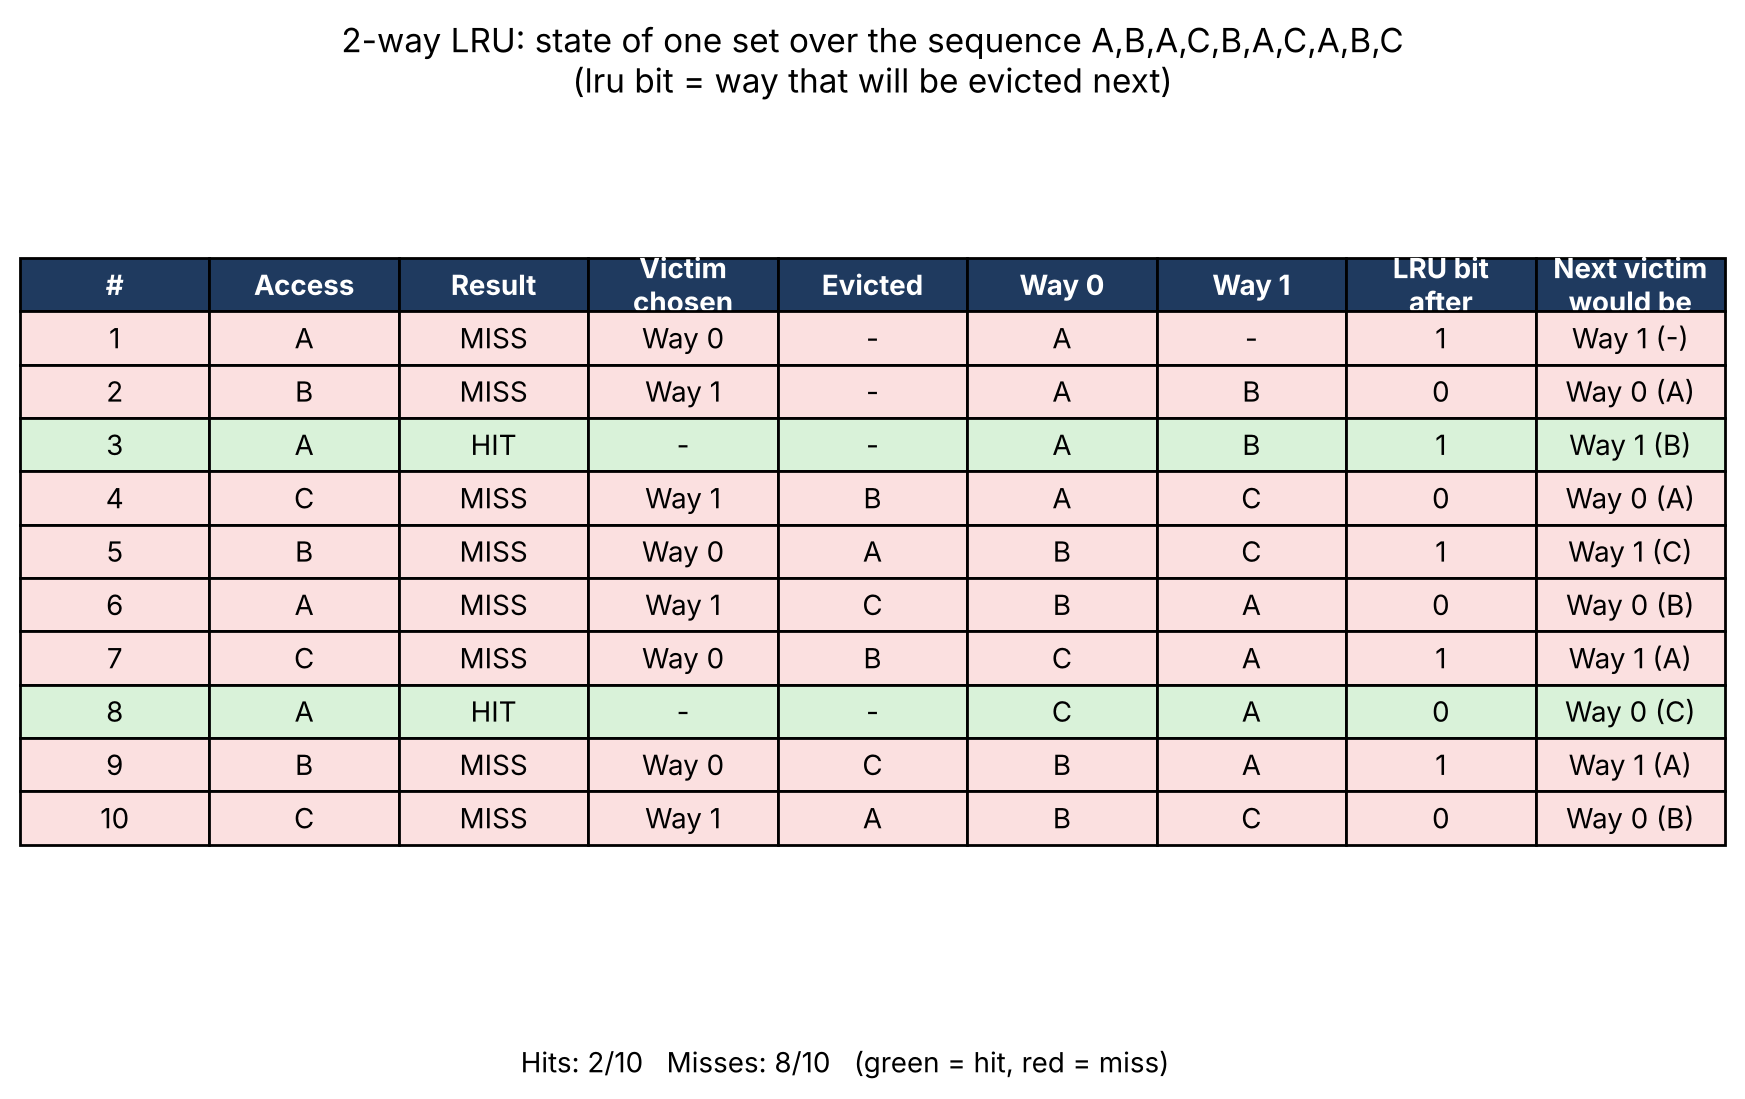
\includegraphics[width=\columnwidth]{lru_sequence.png}
\caption{LRU state transitions across the 10-step reference sequence $A, B, A, C, B, A, C, A, B, C$ in Set~0 (\texttt{docs/img/lru\_sequence.png}).}
\label{fig:lru_sequence}
\end{figure}

The directed testbench \texttt{tb/tb\_lru\_directed.v} verifies this logic through 10 directed test cases, verifying cold allocation priority, eviction protection on hits, multi-set isolation, and write-hit LRU updates, all passing with zero errors.

\subsection{Controller Finite State Machine (FSM) and Timing Analysis}
The cache controller implements a streamlined 4-state Mealy/Moore FSM:
\begin{enumerate}
    \item \textbf{STATE\_IDLE (3'b000):} Awaits active \texttt{cpu\_req}. Latch address, write-enable, and write data into \texttt{req\_addr}, \texttt{req\_we}, \texttt{req\_wdata}.
    \item \textbf{STATE\_LOOKUP (3'b001):} Evaluates continuous tag comparisons. On a read hit, routes data word to \texttt{cpu\_rdata}, pulses \texttt{cpu\_ready = 1}, updates LRU, and returns to \texttt{IDLE} in \textbf{2 clock cycles (20~ns)}. On a read miss, asserts \texttt{mem\_req = 1} and transitions to \texttt{STATE\_MISS\_FETCH}. On a write, transitions to \texttt{STATE\_WRITE\_THROUGH}.
    \item \textbf{STATE\_MISS\_FETCH (3'b010):} Waits for backing memory acknowledgment (\texttt{mem\_ready}). Collects 4 consecutive burst words into \texttt{refill\_buf[0..3]}, writes the complete block to the victim way, updates valid/tag/LRU, asserts \texttt{cpu\_ready = 1}, and returns to \texttt{IDLE} in \textbf{14 clock cycles (140~ns)}.
    \item \textbf{STATE\_WRITE\_THROUGH (3'b011):} Holds \texttt{mem\_req = 1, mem\_we = 1} to forward store data to memory. On \texttt{mem\_ready}, asserts \texttt{cpu\_ready = 1} and returns to \texttt{IDLE} in \textbf{7 clock cycles (70~ns)}.
\end{enumerate}

\begin{figure}[htbp]
\centering
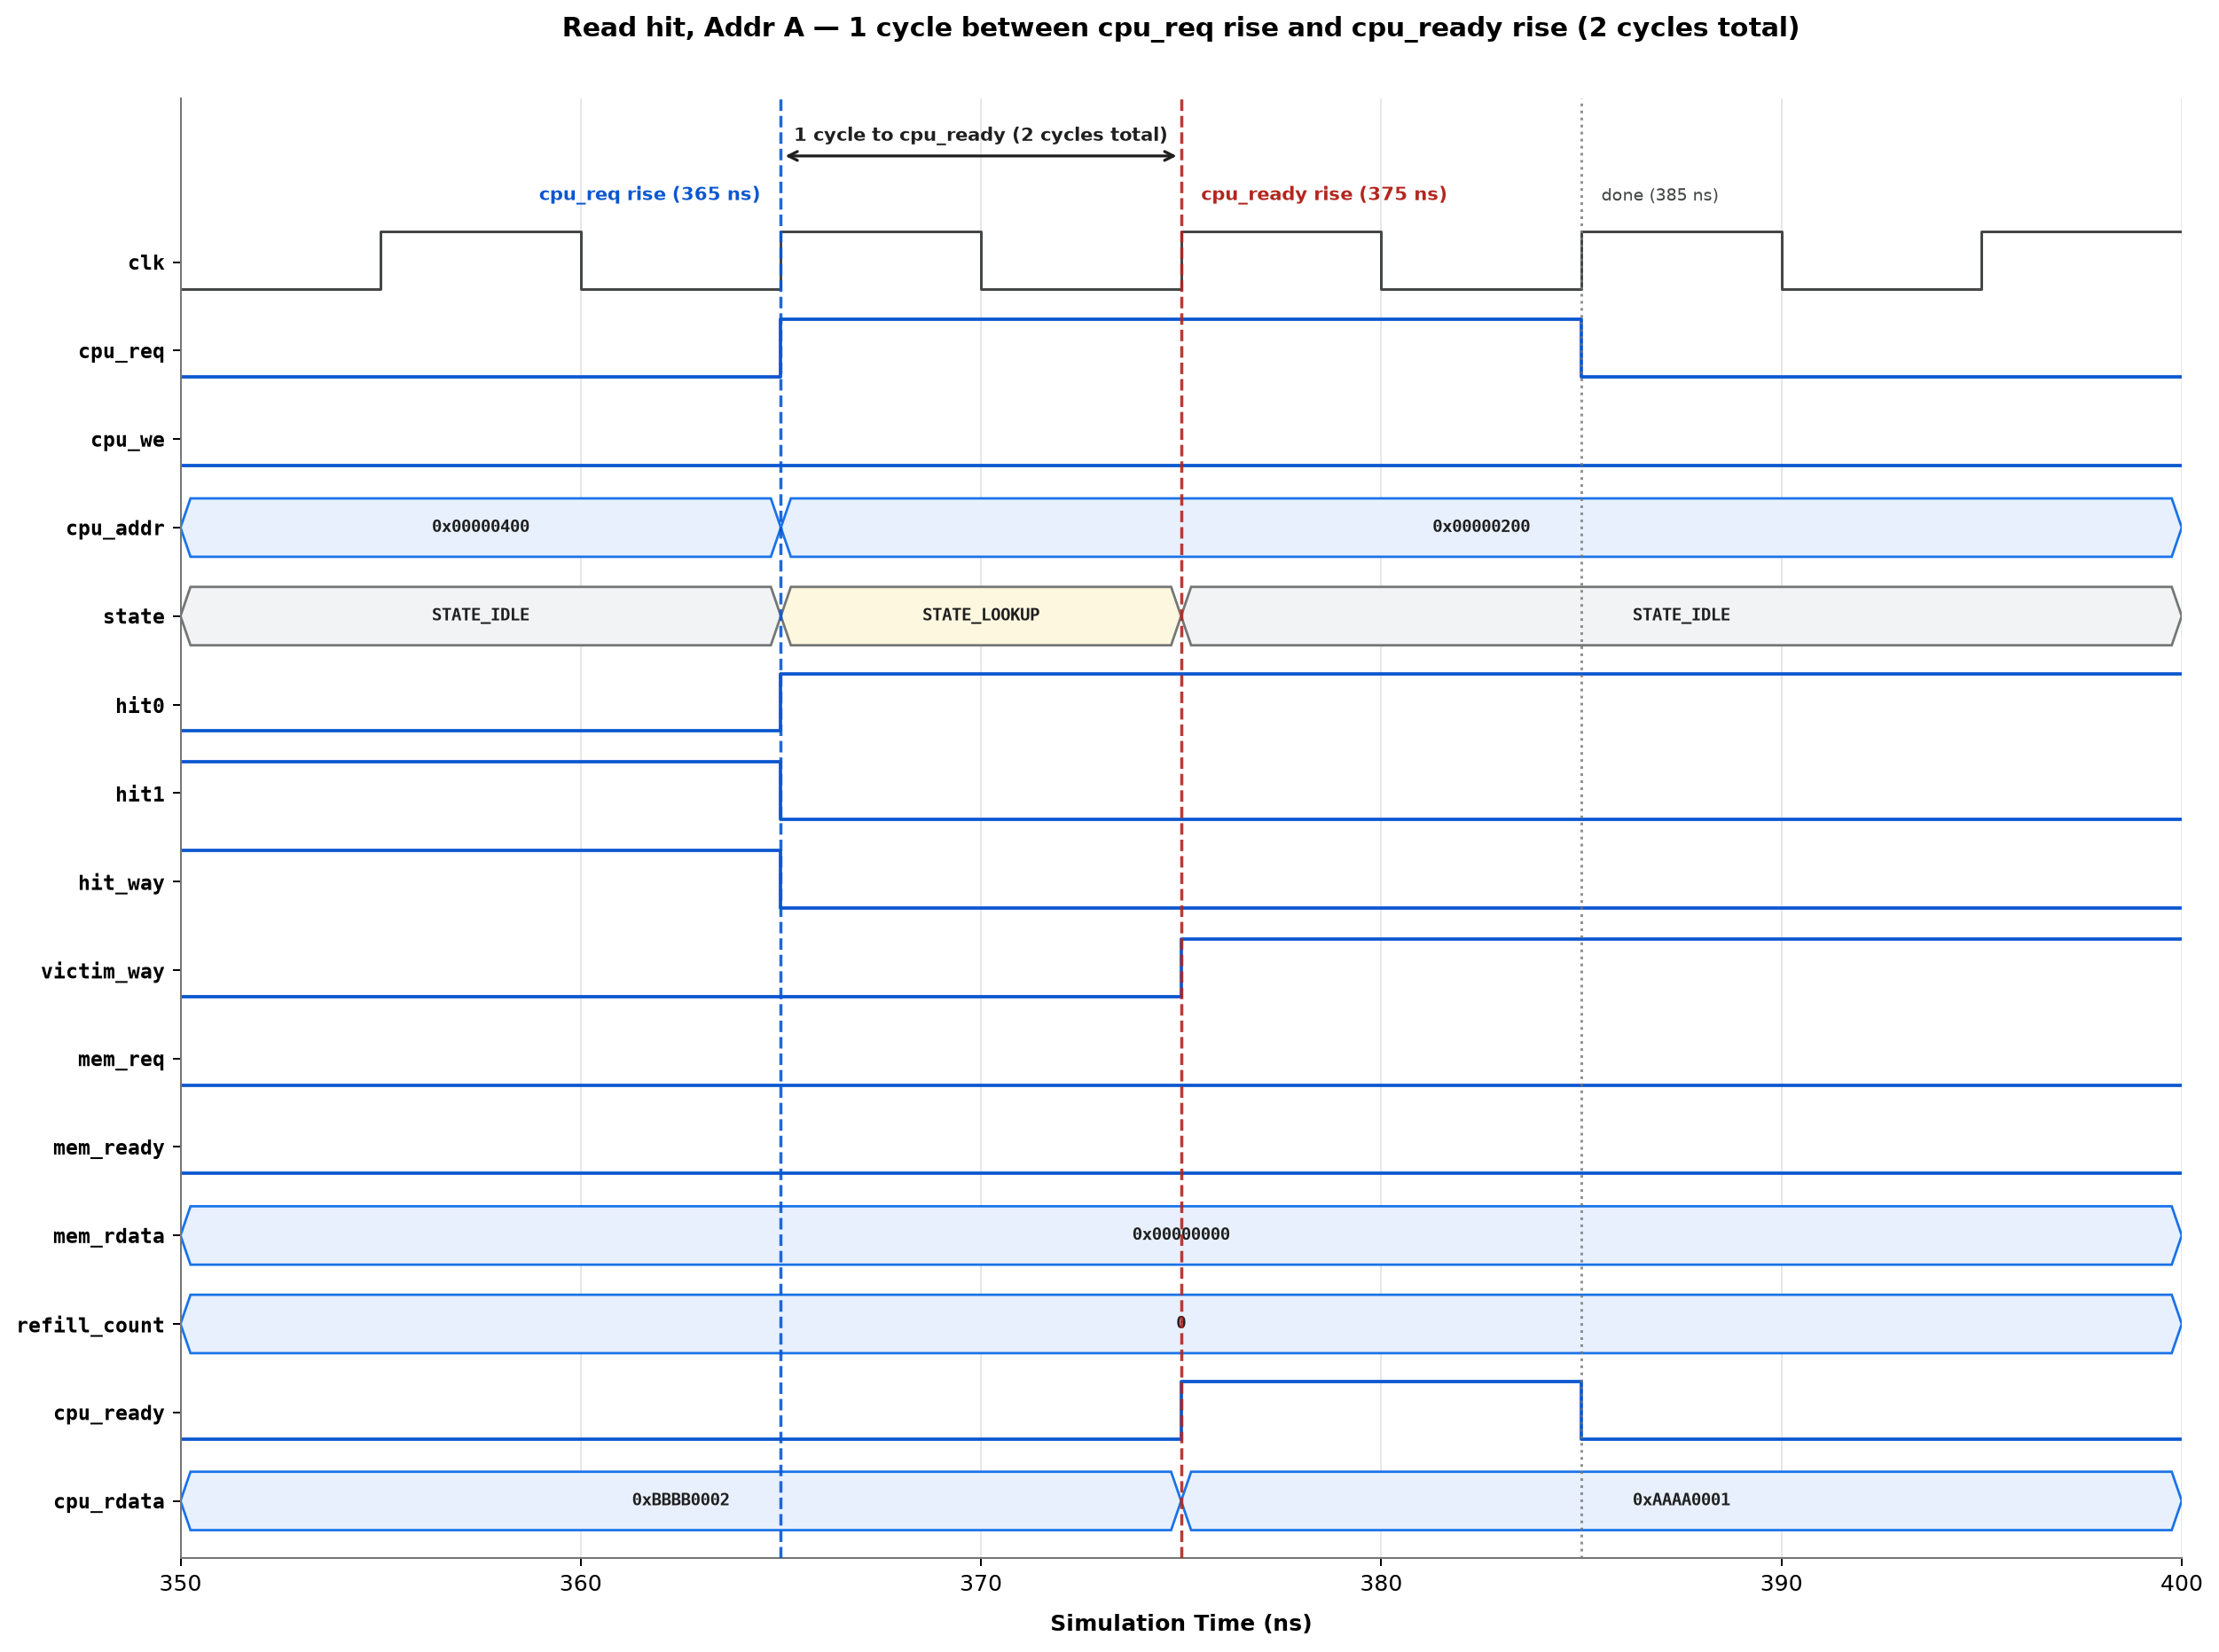
\includegraphics[width=\columnwidth]{waveform_hit.png}
\caption{GTKWave simulation waveform for a 2-cycle read hit (\texttt{docs/img/waveform\_hit.png}).}
\label{fig:wave_hit}
\end{figure}

\begin{figure}[htbp]
\centering
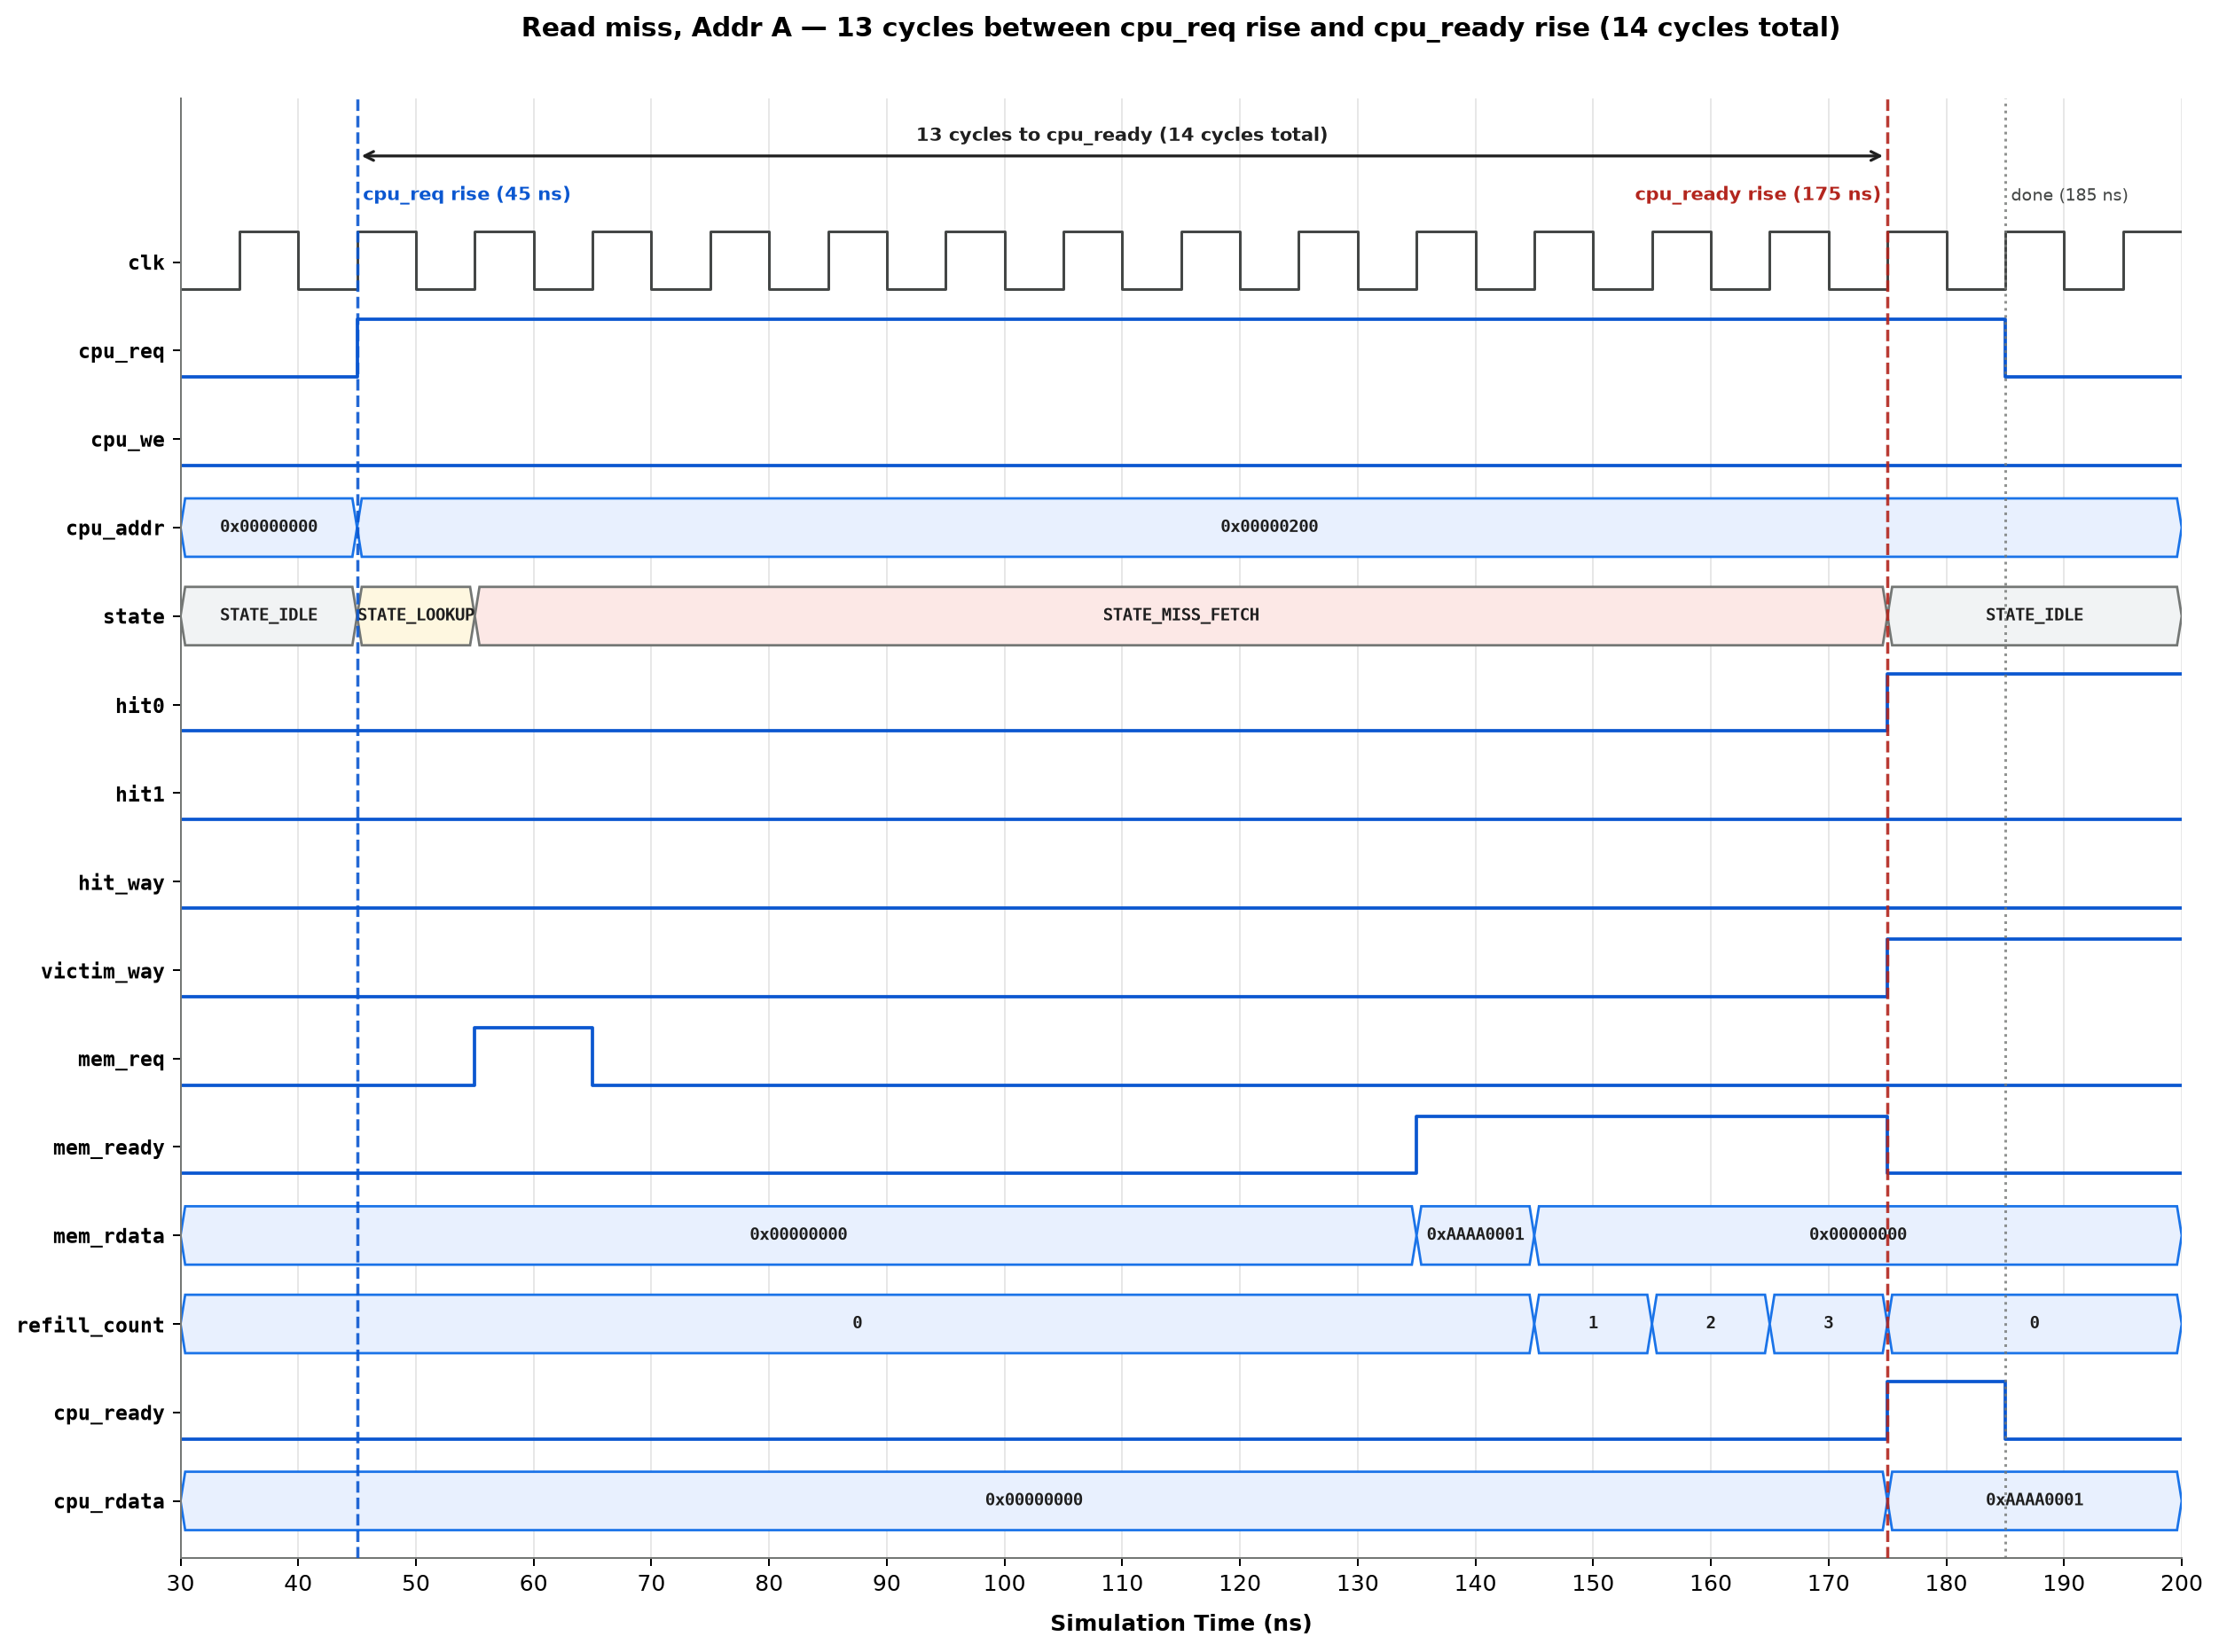
\includegraphics[width=\columnwidth]{waveform_miss.png}
\caption{GTKWave simulation waveform for a 14-cycle read miss refill (\texttt{docs/img/waveform\_miss.png}).}
\label{fig:wave_miss}
\end{figure}

\subsection{Write Policy: Write-Through No-Write-Allocate}
In both cache architectures, memory store transactions are governed by a \textbf{Write-Through, No-Write-Allocate} policy:
\begin{itemize}
    \item \textbf{Write Hit:} Updates the internal cache data word and LRU bit, simultaneously issuing a store transaction across the memory bus.
    \item \textbf{Write Miss (No-Write-Allocate):} Forwards the write directly to main memory without allocating a cache block. This prevents cache pollution from write-only data streams.
    \item \textbf{Trade-off:} Guarantees cache-memory coherence without dirty bits or write-back buffers, but stalls the processor for 7 cycles on every write.
\end{itemize}

\subsection{Fair Comparison Methodology}
To ensure that performance variations stem solely from set associativity, strict architectural controls are enforced:
\begin{itemize}
    \item \textbf{Capacity \& Block Size Parity:} Both caches provide exactly 1024 Bytes of user data organized as 16-Byte blocks (64 blocks total).
    \item \textbf{Identical Memory Timing:} Both caches interface with the identical memory controller (\texttt{rtl/main\_memory.v}) with $\text{RD\_LAT} = 8$ and $\text{WR\_LAT} = 4$.
    \item \textbf{Active Cycle Accounting:} Cycles are counted strictly during CPU service intervals (\texttt{cpu\_req} asserted to \texttt{cpu\_ready} asserted).
    \item \textbf{Golden Memory Cross-Check:} \texttt{tb/tb\_compare.v} validates every read output against an architectural golden memory array. Across all 3,136 transactions, zero data mismatches occurred.
\end{itemize}

\subsection{Evaluation Traces \& Locality Patterns}
Nine deterministic synthetic workloads generated by \texttt{scripts/gen\_traces.py} exercise varied locality dimensions:
\begin{enumerate}
    \item \texttt{seq\_stream} (256 accesses): Linear stride=4 traverse 1024B. Spatial locality only; 75.00\% hit rate.
    \item \texttt{small\_loop} (640 accesses): 256B loop repeated 10 times. Fits in cache; 97.50\% hit rate.
    \item \texttt{pingpong} (200 accesses): Alternates between 2 addresses mapping to Set~2. 2-way achieves 99.00\%; direct thrashes at 0.00\%.
    \item \texttt{cyclic3} (300 accesses): 3 addresses cyclically accessed in Set~3. 3-way working set defeats 2-way LRU; 0.00\% hit rate for both.
    \item \texttt{strided} (256 accesses): 64B stride across 8 blocks over 32 passes. 96.88\% hit rate.
    \item \texttt{random} (300 accesses): Pseudorandom word reads across 16~KB space. 7.33\% (2-way) vs 6.00\% (direct).
    \item \texttt{mixed\_rw} (300 accesses): 70\% reads, 30\% writes in 512B hot region. 81.33\% hit rate on both.
    \item \texttt{large\_loop} (384 accesses): 1.5~KB working set (96 blocks) iterated 4 times. Exceeds 1~KB cache. Direct-mapped achieves 25.00\% (4,224 cycles); 2-way LRU suffers 0.00\% (5,376 cycles).
    \item \texttt{hot\_stream} (400 accesses): 128B hot region (70\%) mixed with 2~KB sequential stream (30\%). 2-way achieves 90.75\% (1,244 cycles) vs 86.75\% (1,436 cycles) for direct.
\end{enumerate}

\section{Results \& Comparative Analysis}

\subsection{Full Benchmark Results Table}
Table~\ref{tab:results} summarizes cycle-accurate simulation results across all 9 workloads at default baseline latency ($\text{RD\_LAT}=8, \text{WR\_LAT}=4$).

\begin{table*}[htbp]
\centering
\caption{Comprehensive Benchmark Results across 9 Workloads (Source: \texttt{results/results.csv})}
\label{tab:results}
\begin{tabular}{llrrrrrl}
\toprule
\textbf{Trace Name} & \textbf{Design} & \textbf{Accesses} & \textbf{Hits} & \textbf{Misses} & \textbf{Hit Rate} & \textbf{Cycles} & \textbf{Key Architectural Observation} \\
\midrule
\texttt{seq\_stream} & 2-Way LRU & 256 & 192 & 64 & 75.00\% & 1,280 & Compulsory misses (1 per 4-word block); spatial parity \\
\texttt{seq\_stream} & Direct-Mapped & 256 & 192 & 64 & 75.00\% & 1,280 & Compulsory misses (1 per 4-word block); spatial parity \\
\midrule
\texttt{small\_loop} & 2-Way LRU & 640 & 624 & 16 & 97.50\% & 1,472 & 256B working set fits in 1KB cache; temporal reuse \\
\texttt{small\_loop} & Direct-Mapped & 640 & 624 & 16 & 97.50\% & 1,472 & 256B working set fits in 1KB cache; temporal reuse \\
\midrule
\texttt{pingpong} & 2-Way LRU & 200 & 198 & 2 & \textbf{99.00\%} & \textbf{424} & 2 conflicting addresses fit in 2 ways (\textbf{6.6$\times$ faster}) \\
\texttt{pingpong} & Direct-Mapped & 200 & 0 & 200 & \textbf{0.00\%} & \textbf{2,800} & Catastrophic thrashing on Set 2 with alternating lines \\
\midrule
\texttt{cyclic3} & 2-Way LRU & 300 & 0 & 300 & 0.00\% & 4,200 & 3-way cyclic access defeats 2-way LRU \\
\texttt{cyclic3} & Direct-Mapped & 300 & 0 & 300 & 0.00\% & 4,200 & Complete thrashing on single cache line \\
\midrule
\texttt{strided} & 2-Way LRU & 256 & 248 & 8 & 96.88\% & 608 & 64B stride hits every 4th set; loop retained \\
\texttt{strided} & Direct-Mapped & 256 & 248 & 8 & 96.88\% & 608 & 64B stride hits every 4th set; loop retained \\
\midrule
\texttt{random} & 2-Way LRU & 300 & 22 & 278 & \textbf{7.33\%} & \textbf{3,936} & Slight associativity benefit under uniform random \\
\texttt{random} & Direct-Mapped & 300 & 18 & 282 & \textbf{6.00\%} & \textbf{3,984} & Absence of spatial/temporal locality \\
\midrule
\texttt{mixed\_rw} & 2-Way LRU & 300 & 244 & 56 & 81.33\% & 1,499 & 70\% read / 30\% write; Write-Through verified \\
\texttt{mixed\_rw} & Direct-Mapped & 300 & 244 & 56 & 81.33\% & 1,499 & 70\% read / 30\% write; Write-Through verified \\
\midrule
\texttt{large\_loop} & 2-Way LRU & 384 & 0 & 384 & \textbf{0.00\%} & \textbf{5,376} & 3 blocks/set: catastrophic cyclic thrashing across all sets \\
\texttt{large\_loop} & Direct-Mapped & 384 & 96 & 288 & \textbf{25.00\%} & \textbf{4,224} & 32 non-colliding lines hit repeatedly (\textbf{Direct is better}) \\
\midrule
\texttt{hot\_stream} & 2-Way LRU & 400 & 363 & 37 & \textbf{90.75\%} & \textbf{1,244} & 2nd way shields hot data from cold stream (\textbf{13.4\% faster}) \\
\texttt{hot\_stream} & Direct-Mapped & 400 & 347 & 53 & \textbf{86.75\%} & \textbf{1,436} & Cold stream evicts hot lines on alias collisions \\
\bottomrule
\end{tabular}
\end{table*}

\begin{figure}[htbp]
\centering
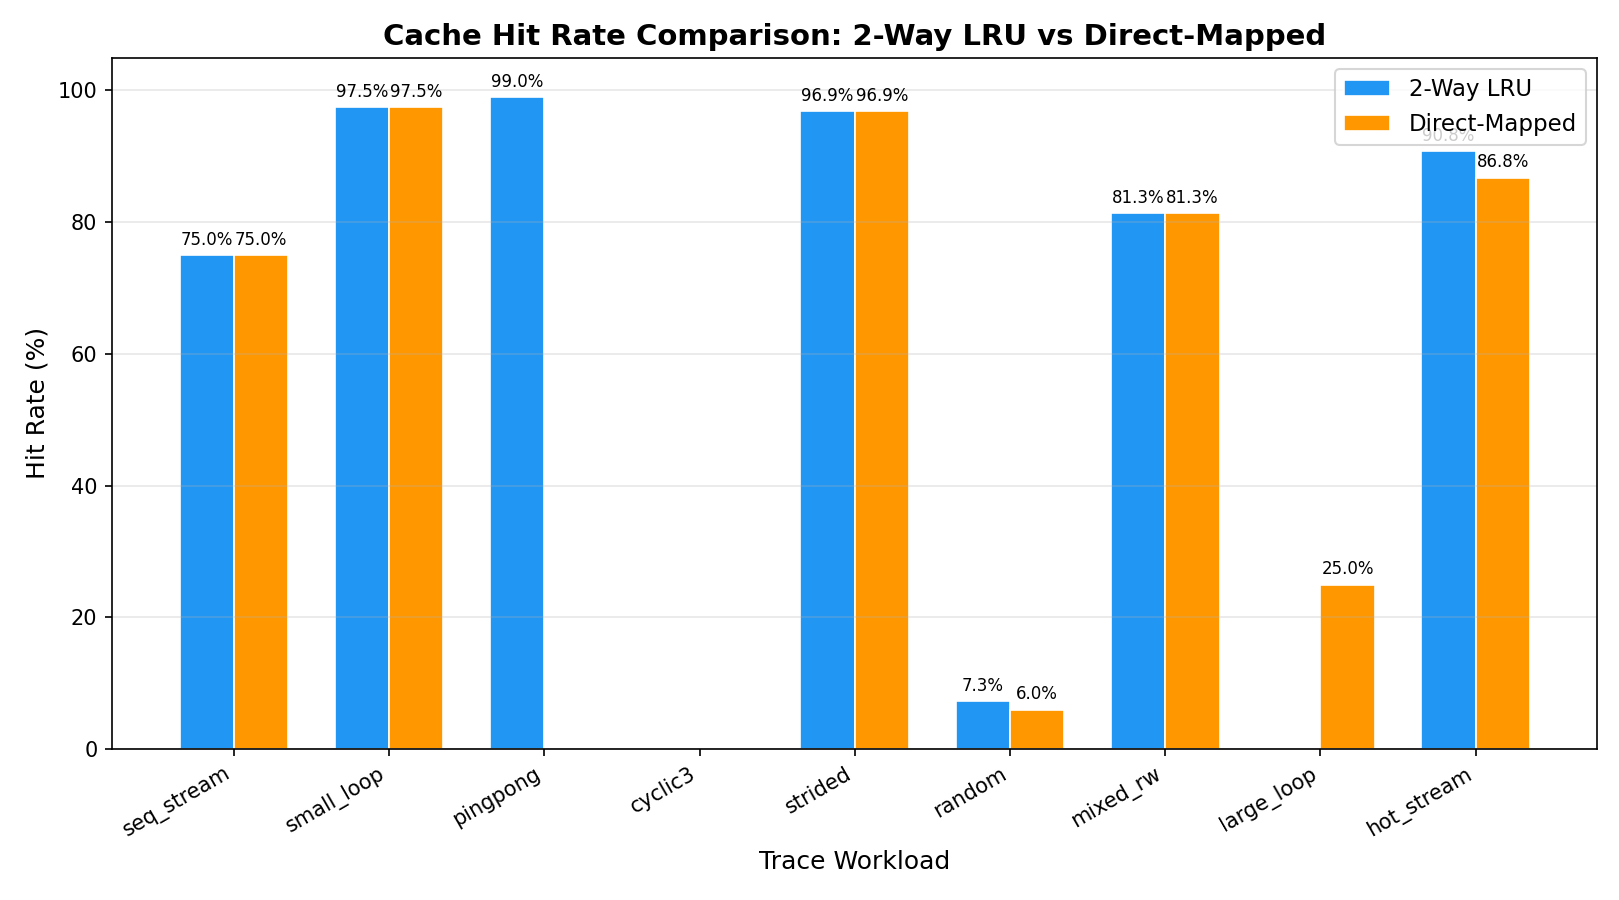
\includegraphics[width=\columnwidth]{hit_rate.png}
\caption{Hit rate comparison across all 9 synthetic benchmarks (\texttt{docs/img/hit\_rate.png}).}
\label{fig:hit_rate}
\end{figure}

\begin{figure}[htbp]
\centering
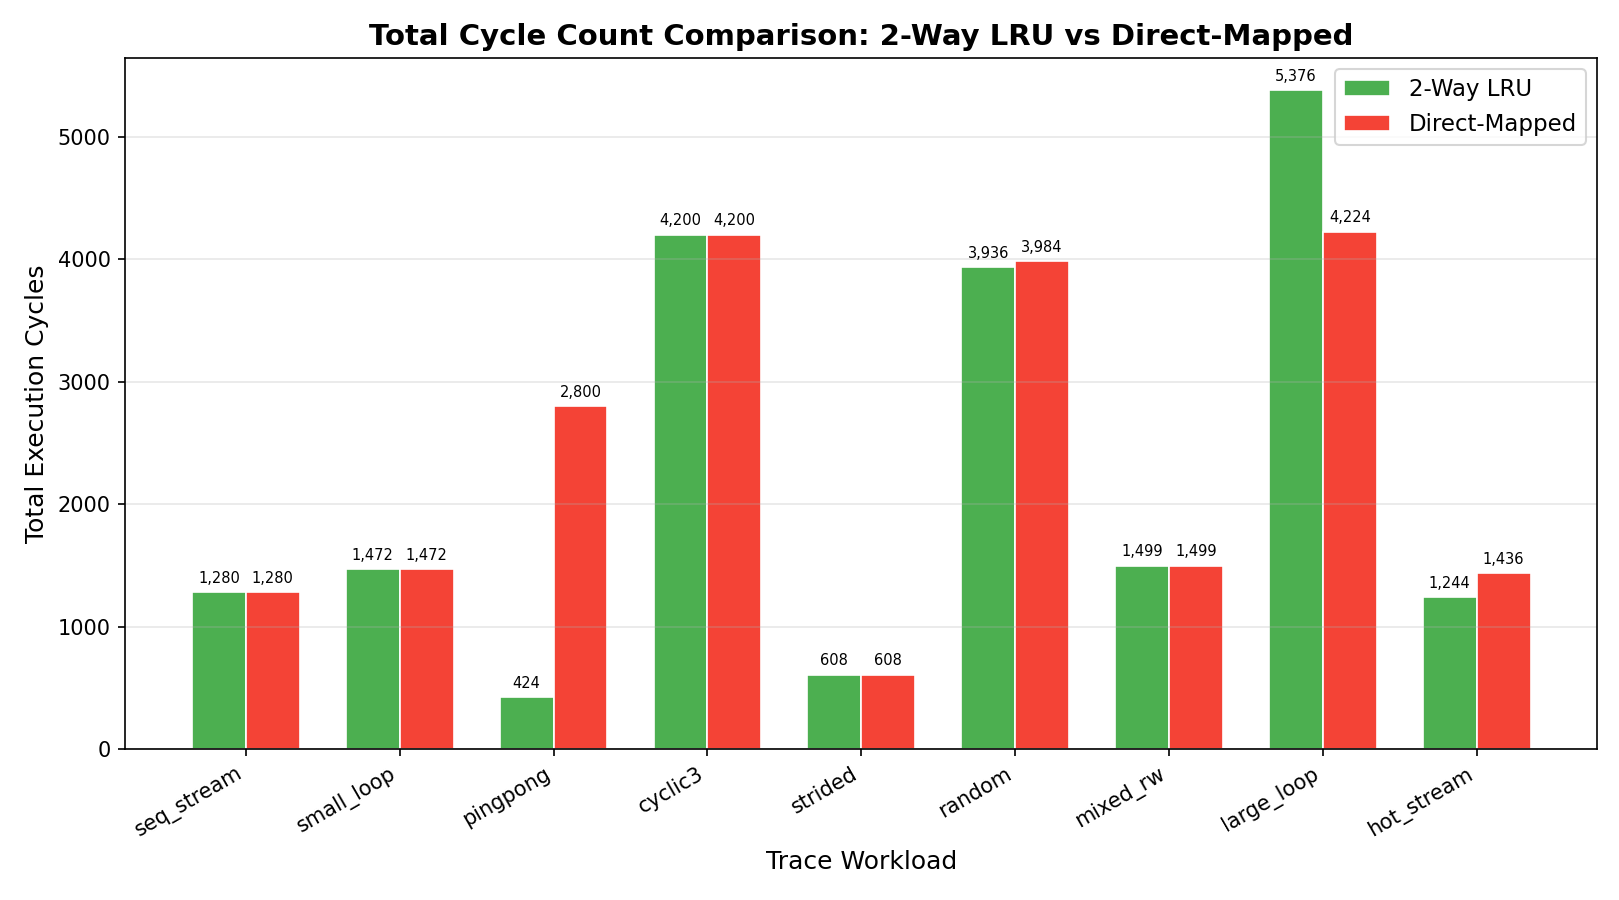
\includegraphics[width=\columnwidth]{cycles.png}
\caption{Active execution cycles across all 9 synthetic benchmarks (\texttt{docs/img/cycles.png}).}
\label{fig:cycles}
\end{figure}

\subsection{Analytical Cycle Verification}
For all read-only workloads, measured execution cycles match the analytical formula to the exact cycle:
\begin{align*}
    \text{Total Cycles} = (\text{Hits} \times 2) + (\text{Misses} \times 14)
\end{align*}
For \texttt{mixed\_rw} (197 reads: 165 hits, 32 misses; 103 writes):
\begin{align*}
    \text{Total Cycles} = (165 \times 2) + (32 \times 14) + (103 \times 7) = 1,499\text{ cycles} \quad \checkmark
\end{align*}

\subsection{Latency Sensitivity Analysis}
Varying read latency $\text{RD\_LAT} \in \{4, 8, 16\}$ demonstrates that cycle variance scales linearly:
\begin{align*}
    \Delta\text{cycles} = (\text{read misses}) \times (\Delta\text{RD\_LAT})
\end{align*}
On \texttt{pingpong}, because the 2-way cache incurs only 2 cold misses, doubling read latency from 8 to 16 cycles increases total cycles by merely 3.8\% (424 to 440 cycles). For the direct-mapped cache, 200 conflict misses cause a 57.1\% cycle inflation (2,800 to 4,400 cycles).

Varying write latency $\text{WR\_LAT} \in \{2, 4, 8\}$ illustrates that under unbuffered write-through, store operations stall execution by $\Delta\text{cycles} = (\text{writes}) \times (\Delta\text{WR\_LAT})$. On \texttt{mixed\_rw}, shifting $\text{WR\_LAT}$ from 4 to 2 reduces execution by exactly $103 \times (-2) = -206$ cycles, while increasing to 8 adds $103 \times (+4) = +412$ cycles.

\subsection{Hardware Synthesis \& Resource Utilization}
Both designs were evaluated under generic technology elaboration with Yosys. Because behavioral Verilog arrays infer registers, storage allocation is dominated by memory flip-flops:
\begin{itemize}
    \item \textbf{Direct-Mapped Baseline:} Data storage: $64 \times 128\text{b} = 8,192\text{ bits}$; Tag storage: $64 \times 22\text{b} = 1,408\text{ bits}$; Valid storage: $64 \times 1\text{b} = 64\text{ bits}$. Total architectural storage: \textbf{9,664 register bits}.
    \item \textbf{2-Way Set-Associative Cache:} Data storage: $32 \times 2 \times 128\text{b} = 8,192\text{ bits}$; Tag storage: $32 \times 2 \times 23\text{b} = 1,472\text{ bits}$; Valid storage: $64\text{ bits}$; LRU replacement: $32 \times 1\text{b} = 32\text{ bits}$. Total architectural storage: \textbf{9,760 register bits} (+96 bits, a 1.0\% increase).
\end{itemize}
The primary area and delay cost of 2-way associativity stems from combinational logic: doubling comparator count (two 23-bit comparators vs one 22-bit comparator), 32-bit hit-way multiplexing in the read critical path, and priority victim selection logic. Vivado FPGA synthesis figures ($F_{\max}$, LUT/BRAM utilization) were not collected in Phase I.

\section{Individual Contributions}
Individual team contributions were determined from the repository commit log (\texttt{git shortlog -sne main}) and merged pull requests:

\begin{table}[htbp]
\centering
\caption{Team Member Contributions and Verified Commits}
\label{tab:contrib}
\begin{tabular}{p{1.1cm}p{1.9cm}p{2.6cm}c}
\toprule
\textbf{Member} & \textbf{Role} & \textbf{Deliverables \& PR} & \textbf{Commits} \\
\midrule
\textbf{Member 1} & Team Lead \& 2-Way RTL & \texttt{cache\_2way\_lru.v}, report III.A, III.B, III.D; PR \#1 & 24 \\
\textbf{Member 2} & LRU Logic \& Verification & \texttt{tb\_lru\_directed.v}, LRU diagram, report III.C; PR \#6 & 19 \\
\textbf{Member 3} & Baseline \& Memory Model & \texttt{cache\_direct.v}, \texttt{main\_memory.v}, latency study, report III.E, III.F; PR \#7 & 6* \\
\textbf{Member 4} & Traces \& Benchmarks & \texttt{gen\_traces.py} (9 traces), \texttt{tb\_compare.v}, \texttt{plot\_results.py}, report III.G, IV; PR \#8 & 6 \\
\textbf{Member 5} & Report, Synthesis \& Video Lead & Report assembly, IEEEtran package, block diagram script, synthesis summary; active PR & 7 \\
\bottomrule
\end{tabular}
\end{table}

\noindent \textit{*Attribution Flag:} All 6 commits for Member~3 were committed under \texttt{neerajsingh@Neerajs-MacBook-Pro-2.local}. This local address is flagged for correction before final grading submission.

\section{Conclusion}
Phase I of Project 7 achieved complete architectural design, cycle-accurate functional verification, and performance evaluation for a 1~KB 2-way set-associative cache and direct-mapped baseline.

The empirical findings confirm that:
\begin{enumerate}
    \item Set associativity provides dramatic performance benefits on conflict-heavy workloads (\texttt{pingpong}), improving hit rate from 0.00\% to 99.00\% and reducing execution cycles by 6.6$\times$ (424 vs 2,800 cycles).
    \item When working sets exceed associativity cyclically (\texttt{cyclic3}), LRU exhibits catastrophic thrashing, achieving 0.00\% hits for both caches.
    \item Direct-mapped caches can outperform 2-way LRU on loops sized between $C$ and $2C$ capacity (\texttt{large\_loop}, 1.5~KB working set), where direct-mapped achieves a 25.00\% hit rate (4,224 cycles) while 2-way LRU thrashes at 0.00\% (5,376 cycles) due to non-colliding modulo-64 line survivals.
    \item Unbuffered write-through operations impose heavy bus stall overheads (7 cycles per store), as confirmed by 721 stall cycles in \texttt{mixed\_rw}.
\end{enumerate}

\textbf{Methodological Limitations:} Evaluations were conducted via cycle-accurate RTL simulation with generic Yosys elaboration. Hit-time clock degradation due to comparator and multiplexer propagation delays and FPGA post-routing $F_{\max}$ were not measured. Furthermore, Phase II implementation plans (including write-back dirty bit tracking, multi-level hierarchy, or FPGA deployment on Vivado) remain \textbf{TO CONFIRM}.

\bibliographystyle{IEEEtran}
\bibliography{references}

\end{document}
